\documentclass[msc]{ppgccufmg}

\usepackage[english]{babel}
\usepackage[utf8]{inputenc}
\usepackage[T1]{fontenc}
\usepackage{type1ec}
\usepackage{graphicx}
\usepackage{xcolor}
\usepackage[a4paper,
  english,
  bookmarks=true,
  bookmarksnumbered=true,
  linktocpage,
  colorlinks,
  citecolor=black,
  urlcolor=black,
  linkcolor=black,
  filecolor=black,
  ]{hyperref}
\usepackage[square]{natbib}

\begin{document}

\ppgccufmg{
    title={Automatic pain assessment in fetuses through transfer learning},
    authorrev={Oliveira, Thiago Melo de},
    cutter={D1234p},
    cdu={519.6*82.10},
    university={Federal University of Minas Gerais},
    course={Computer Science},
    portugueseuniversity={Universidade Federal de Minas Gerais},
    portuguesecourse={Ciência da Computação},
    address={Belo Horizonte},
    date={2020-03},
    advisor={Nivio Ziviani},
    coadvisor={Adriano Veloso},
    abstract={Abstract}{abstract},
    dedication={dedicatoria},
    ack={agradecimentos},
    keywords={Insert Keywords Here},
    epigraphtext={Truth and lie are opposite things.}{Unknown},
}

\chapter{Introduction}

The International Association for the Study of Pain (IASP) defines pain as ``an unpleasant sensory and emotional experience associated with actual or potential tissue damage, or described in terms of such damage'' \citep{merskey1994classification}. The definition accompanying notes also establishes that ``the inability to communicate verbally does not negate the possibility that an individual is experiencing pain and is in need of appropriate pain-relieving treatment.''

As newborns are unable to self-report pain, its diagnosis is much harder when compared to adults. Thus, specialists have used non-verbal responses like facial expressions, crying sounds, and movements, alongside physiological measurements for better pain assessment. These methods have been tested and found to be reliable indicators of pain. Several observational scales have been published and verified based on them, such as the Neonatal Infant Pain Scale (NIPS) \citep{Lawrence1993}, and the Neonatal Facial Coding System (NFCS) \citep{Grunau1998}.

In the case of fetuses, as we have even more restrict methods of pain assessment, diagnosis becomes more difficult. Fortunately, some recent studies have shown the feasibility of applying these pain scales on a fetus through the use of 4-D (four-dimensional) ultrasound images \citep{bernardes2018feasibility}. This process allowed the monitoring of facial expressions on a fetus while they were exposed to noxious stimuli like an anesthetic puncture.

With recent advances in Artificial Intelligence (AI), the capacity of machines to detect patterns in images has largely improved, which consequently allowed for its application in innumerous scenarios. Hence, these techniques could also be useful for pain assessment by helping to match the patterns of facial expressions that are common indicators of pain.

\section{Motivation}

With studies showing that fetuses beyond a certain age can also experience pain \citep{Derbyshire2006, Derbyshire2020}, early identification of this discomfort can be valuable in many situations. 

One example is intrauterine surgery, which may be of significant benefit in the future development and survival of the fetus. Early correction, prior to birth, of congenital problems, will likely increase the odds of a healthy baby. These procedures, however, are quite invasive to the fetus and could eventually cause harm. The assessment of pain during the intrauterine life of a fetus is, therefore, a task with the potential of bringing significant improvements to fetus life quality. 

Another critical topic is abortion. In the United States, a 2016 law from the state of Utah determines that women seeking abortion 20 weeks or more into pregnancy will first have to be given anesthesia or painkillers \citep{healy2016nytimes}. This procedure is intended not for them but the fetus. 

This topic involves much ethical debate, as the exact week when a fetus starts experiencing pain is not well defined, and at the same time, abortion is only legal until a particular week \citep{Derbyshire2006}. So discussion arises not only if the fetus can or can not experience pain, but also as it may be the case that fetuses can only experience pain after weeks in which abortion is no longer possible. Evidence on the presence of pain in this scenario would be a significant contribution in such a delicate situation and may assist the decision by the doctors and the mother.

For both scenarios, the current standard for assessing pain in infants and fetuses relies on caregivers' observation of specific behaviors such as facial expressions. However, these observations are subject to bias and can be affected by several factors, such as identity, background, culture, and gender, which may lead to inconsistent assessment and treatment of pain. An impartial perspective during the pain assessment process could bring a more realistic and deterministic view on the subject. Hence, computational help would be of great use in finding evidence of pain and in effectively managing it.

\section{Thesis Statement}

Our work developed a learning model capable of automatically detecting the presence of pain in fetuses through the evaluation of their facial expressions in images collected from 4-D ultrasound machines. We have used modern deep learning techniques like transfer learning and data augmentation to find the best model. Our results demonstrated the effectiveness of applying such methods in the fetal domain and, to the best of our knowledge, is the first work attempting to do so.

\section{Contributions}

As fetuses have been shown to respond to stimuli like anesthesia with facial expressions indicating pain, the goal of this work is to help automate the pain assessment process and to generate unbiased evidence of pain. We have developed a process capable of detecting the presence of pain from images collected from 4-D ultrasound machines.

If this system is eventually integrated into the ultrasound machine itself, it will bring many benefits, such as the monitoring of anesthetic procedures efficacy, much like what it is done in adults. As an example, if the surgeon detects that after the first anesthesia, the fetus still shows signs of pain, he will be able to make better decisions and apply another one if necessary.

This work also opens the way to explore the evolution of pain-related facial responses during fetal development. Considering that after the 20th gestational week, fetuses start to develop brain structures capable of showing signs of pain, this model would, therefore, allow for continuous monitoring of pain across time.

In summary, our main contributions are:

\begin{itemize}
    \item We have created a systematic procedure for collecting and processing images of a fetus from videos of 4-D ultrasound machines. This procedure is also capable of detecting their facial landmarks. From this procedure, we have created a labeled database consisting of 230 images of 15 fetuses with facial expressions while in the manifestation of pain and two other control conditions. To the best of our knowledge, no such database existed.
    
    \item We have developed a learning model capable of detecting the presence of pain indicators from images of a fetus's face. We believe this is good evidence towards an unbiased pain assessment process. This novel approach has the potential to improve the pain assessment process significantly on fetuses. It would facilitate pain management by the doctors and caregivers and could even be the first indicator of discomfort or distress, leading to earlier intervention if necessary.
    
    \item We have shown that transfer learning with a network pre-trained with the face recognition task transfers well to fetus images even though the domain is different. We have achieved an area under the ROC curve of 0.69 on the classification task between pain and non-pain.
\end{itemize}

\section{Organization}

The rest of this dissertation is structured as follows. First, Chapter 2 discusses related work in pain assessment. Chapter 3 introduces some background concepts on deep learning, necessary to further understand our work. Chapter 4 describes the fetal pain assessment study, and also introduces our dataset. Chapter 5 follows with our methodology, including our learning model. Then, Chapter 6 describes our validation process, as well as our experimental results. Chapter 7 concludes the dissertation and present future work possibilities.
\chapter{Related Work}

In this chapter, we present the most relevant research results that guided our work, exposing the methodologies used by the authors and how they correlate to ours. Research on automatic pain assessment has a significant intersection between the medical field and applied machine learning both for fetuses and infants \citep{Bellieni2012, ZamzmiPGKSA16}. Thus, we start by exploring the signs of pain in infants and fetuses, their main indicators, the available pain scales to measure them, and automatic methods of assessment. We conclude the chapter by explaining how our work is different from the mentioned ones, as we explore automatic pain assessment from a novel perspective with fetuses.

\section{Pain}

Pain is a universal form of distress present in humans and some other animals. Acute and chronic pain is very typical in the population and constitutes widespread public health problems \citep{Goldberg2011}. Its prolonged presence could cause many adverse consequences, including psychological effects, which is especially true in the case of neonates and fetuses.

The study of neonatal pain appears to have begun as early as the 1870s when Dr. Flechsig proposed it was unlikely that neonates could feel pain because their neuronal myelination was not complete \citep{cope1998neonatal}. Charles Darwin's book written a couple of years later agreed with this view, as he wrote that ``infant's pain expressions were related to reflexes only'' \citep{darwin1872expression}. Even in the 1950s, some pediatric surgeries were still performed without analgesia and anesthesia \citep{cope1998neonatal}.

It was only in the early 1980s that the first fetal surgery was performed by Dr. Michael Harrison \citep{Harrison1982}. The fetus to be operated had a blockage in the urinary tract that caused the kidney to dangerously extend, which is a condition known as congenital hydronephrosis. A vesicostomy was conducted to correct this issue by placing a catheter in the fetus to allow the urine to be released normally.

Further progress has been made in the years since this first operation, as advances in imaging technology and in surgery techniques allowed additional abnormalities to be treated and for less invasive forms of fetal surgical intervention to be performed.

Even though the cases in which fetal surgery is necessary are relatively rare, it has become the standard form of intervention in some abnormalities like myelomeningocele, as shown by the Management of Myelomeningocele (MOMs) Trial \citep{Adzick2011}. The study compared outcomes of in utero repair (before birth) with standard postnatal repair (after birth). The conclusion was that prenatal repair might result in better neurological function than repair deferred until after delivery.

The study of fetal surgery is tightly coupled with the one of fetal pain. \cite{Fisk2001}, for instance, evaluated the effect of opioid analgesia on fetal hormonal stress responses to intrauterine needling and showed that fentanyl, an opioid commonly used for pain medication and anesthesia, does attenuate the fetal stress responses.

Later on, \cite{vandeVelde2012} studied fetal reactions to painful stimuli and showed that painful interventions could have long-term effects on them. This study also concluded that adequate pain relief during potentially painful procedures is recommended. 

These conclusions also affect anesthesiologists, as \cite{Devoto2017} shows that fetal pain is among their primary concerns during fetal surgery for myelomeningocele. Considering these procedures are so delicate, fetal pain assessment and management are of fundamental help, which leads research to the study of pain detection through the use of pain indicators.

\subsection{Pain Indicators}

Fetuses and infants can produce different signals of pain, which can be decoded to both identify its presence and to measure its level. These signals come from a variety of sources, such as facial expressions, crying sounds, body movements, physiological indicators, and biological markers \citep{Bellieni2012}. 

Even though we have this many indicators, pain identification is a challenging task as we have the manifestation of the same indicators present in similar feelings, such as anger, hunger, or stress. The recommendation to address this issue is that these indicators should be used in combination with each other \citep{Bellieni2012} because most of the time, their presence alone is not sufficient. 

Crying, for instance, can also be generated by hunger or anger. Therefore it can not be used as a sole indicator of pain. In the past, it was believed that different emotions resulted in different types of crying, but this theory has been refuted as it was later discovered that what causes the difference is not the cause of distress, but rather its intensity. 

Thus, some pain scales combine features of crying with other indicators for pain assessment. Fetuses have been shown to express a homolog of crying \citep{Gingras2005}, which can also be further explored for automatic pain assessment, as shown by \cite{abs-1909-02543}. 

Physiological indicators, on the other hand, have the limitation that they are subject to variations due to underlying illness \citep{sweet1998physiological}. Body movements have also been pointed out to be indicators of pain, as fetuses already present withdrawn reflexes during stressful procedures \citep{Zimmermann1991}, but care must be taken as they can also be misleading as other factors may cause the movements.

Studies have also shown that biological markers like stress hormones (cortisol, adrenaline, and beta-endorphins) are increased in concentration in the blood in the presence of pain \citep{giannakoulopoulos1994fetal}. However, the problem of these indicators is that they depend on results from laboratory tests, which makes it unfeasible to use during clinical trials.

One of the most relevant indicators of pain, not only in adults but also in neonates and fetuses are facial expressions. As suggested by \cite{Yan2006}, a great way of evaluating fetal facial expressions is through the means of 4-D sonography, and as he points out, these studies may be the key to predicting fetal brain function and well-being. Later research by \cite{Reissland2011, Reissland2013} also suggests that, when healthy fetuses mature from 24 to 26 weeks of gestation, their capability of showing complex facial movements increases, and they were even able to observe facial expressions which resemble a face while in pain or distress.

Facial expression indicators are frequently present in pain scales. Several facial movements are usually tracked, such as brow bulge, eye squeeze, nasolabial furrow, and open mouth. The assessment of these manifestations is done by observers, which use pain scales to identify its presence and intensity of pain.

\subsection{Pain Scales}

Various neonatal pain scales were developed using the many indicators mentioned in the previous section. These multidimensional scales are used by caregivers to assess pain with behavioral and physiological indicators. The most common scales are:

\begin{itemize}
    \item Neonatal Infant Pain Scale (NIPS), by \cite{Lawrence1993}
    \item Face, Legs, Activity, Crying and Consolability (FLACC), by \cite{Merkel1996}
    \item Neonatal Facial Coding System (NFCS), by \cite{Grunau1998}
\end{itemize}

These scales were all developed with neonates in mind, as some indicators observations are not easily measured in a fetus. However, recent studies by \citeauthor{bernardes2018feasibility} have reported that the use of the NFCS is feasible to detect pain-related facial expressions compared with the rest condition in a randomized and blinded assessment report. We further discuss this study in Chapter 4.

Nevertheless, the scales also have some limitations, as they are highly dependent on the observant bias, require specific training for proper utilization, and are not able to monitor pain in a continuous manner. Thus developing tools that are capable of doing this job automatically and continuously is highly compelling as they can generate a more consistent pain assessment.

\section{Automatic Pain Assessment}

The development of learning models to automatically assess pain has been a topic of research for a long time. As an example, in the adult's domain, \citep{MauricioCVC19} has achieved remarkable results in identifying spatiotemporal features extracted from video sequences for pain recognition.

The first work attempting to automatically assess pain in newborns emerged in 2004 with the development of the iCOPE database \citep{Brahnam2006}. At the time, neural networks were not as popular and advanced as they are today. The first attempts used traditional techniques such as PCA, LDA, and SVM. Still, the results were satisfactory, and the experimental process they developed is similar to what is used today with more modern techniques. 

The iCOPE database consisted of 216 images from 26 infants being 13 girls and 13 boys. The images were collected in 5 different conditions, a resting baseline, bodily disturbance, an air stimulus on the nose, friction on the external surface of the heel, and the pain of a heel stick. The idea behind using this variety of conditions was to make sure the set of images were representative, but also challenging enough. The five conditions were later divided into two groups for classification: pain and non-pain.

Our work has adopted a similar approach of not having only images of rest and pain, but also a third set of images from other stimuli, which in our case was a vibroacoustic sound stimulus with the intention of causing discomfort, but no pain. 

Their first studies considered the best scenario where the system would be able to train on a fetus and evaluate that same fetus later on. However, as permanence in the baby nursery is quite short, they also had to consider the case where this was not possible. Thus the validation process had to consider the other scenario where the classifier had to be trained beforehand and evaluated on images of a new baby, which was not in the dataset distribution previously.

Given they had a small number of subjects, it was feasible to use a validation strategy known as leave-one-out, which consisted of iterating over every combination of using 25 subjects for training and 1 for testing. We have adopted the same strategy in our work.

\section{Learning Models for Pain Assessment}

As opposed to past work, like \citep{ZhiZGALS18}, which used filters and descriptors to extract features from images, modern approaches in automatic pain assessment of neonates usually make the use of neural networks to achieve state of the art results.

\cite{abs-1807-01631}, for instance, has significantly improved the results in the aforementioned iCOPE dataset, achieving 0.948 of AUC by combining both handcrafted features and features extracted by CNNs.

\cite{SalekinZGKH019} proposed a multi-channel shared network to classify pain from videos by extracting features from facial expressions and body movements. He also contributed with an alternative approach by using convolutional neural networks to extract features from crying sounds \citep{abs-1909-02543}.

% In general, much like the pain scales, a combination of features from different inputs is what tends to work best. 
\chapter{Methodology}

As there are no publically available datasets with images of pain assessment in fetus, our work was developed in conjunction with the group of studies of Fetal Pain Assessment from the Univeristy of São Paulo (USP), which studies pain assessment in fetuses and was responsible for collecting the images.

Videos were recorded in three groups. The first one for control purposes, was just with fetuses in resting conditions. The second one was of fetueses that had to go trough an intra-uterin surgery, and thus needed fetal anesthesia, in this case the exact moment when the needle was applied was recorded. This recorded the reaction of the fetus in pain, and in some cases even crying. Notice that these videos also had images (1) a baseline period defined as the least 30 seconds before the anaesthesia puncture and (2) the 45 seconds immediately after the puncture. Finally the third group of videos was recorded while the fetus was exposed to the sound of horn, this was meant to cause distress but it should be a control group rather different from pain which we expected to differentiate.

Videos were recorded from the 4D Ultrasound machine of the model Voluson E8 by GE. 

We had a total of 15 videos to work with, with 5 from each group.

For the images collected during fetal anesthesia, a second ultrasound machine was placed in the clinical room, as the main one was used for the medical procedure of the puncture and the second one was used to target the fetus face an to monitor its expressions.

These images with fetus in pain conditions were evaluated by 3 professionals with the NFCS scale, and these evaluations could further be used to quantify the amount of pain 

**Image Sampling**

Notice that it is common to have an small number of data to work with as this is a very hard data to collect. Only a small percentage of the fetus have to go trough surgery prior to birth, and thus fetal anesthesia is a relatively rare procedure. Other studies also have a small N, like these ones ... 

In order to deal with the limited amount of data, we've decided to deal with this problem in another dimension. We reduced the space from videos to images. In orther to do this, we decided to sample the videos at the hate of every 1 second. With this processes we created a total of XXXX images.

But as the images were recorder from ultrasound machines, they depend on the calibration by the doctors in orther to capture the exact section in the 3 dimensional space where the fetus face is. Because of this, it is common for this type of image to have a lot of noise, and thus some of the sampled images did not contain a clear face of the fetus. This was a problem, as we had a significant number of images, and manual selection would not only hard by non deterministic.

So in orther to overcome this issue, we decided to use a neural network capable of detecting facial landimarks, like the nose, the mouth and the eyes. The network we used was the MTCNN \cite{} which was originally developed to recognize X. But it worked surprisingly well in our domain, even though the images had a quite different characteristics.

With this process, we were able to filter out our dataset of images from XXXX to YYYY, and were sure the images contained a clear face. The network also returned a confidence number of which it found the face in the image, and we've used only confidences of over 95%, which on manual inspection was very reliable, with just 6 errors that were removed manually.

With the position of the facial landmakrs, another process was to crop the images around the face of the fetus. This cropping is done just by adding a padding to the places were the image was. This process is also available trough the MTCNN library, and we can also add face alignement. This way, we avoid the blurred surrounding around the fetus wich contains fragments of the womb and other non distinguishable parts. 

At this point, manual inspection was needed in other to separate the images back into the three groups. With the resting images, it was easy as all the frames were from resting positions. But with the ones from anestheasia and from the horn we had to split the data between before the stimulus and after it. This was not a though process as we knew exactly when the stimuli was applied and a clear difference in the facial expression could be noted. 
\chapter{Deep Learning Models for Fetal Pain Assessment}

In this chapter, we present some background topics recommended for a better understanding of our work and later explain the methodology that was used to conduct our experiments.

\section{Background}

In the task of image classification, traditional machine learning algorithms required hand-engineered features, like filters and descriptors, which were meant to extract information from the images to be used as an input for algorithms. These algorithms would then be trained to find patterns in these features capable of distinguishing between different classes.

Neural networks, on the other hand, have the advantage of being able to learn these features directly from the data, which makes the process of feature engineering a lot simpler and achieves better results in most cases. Furthermore, the recent advances in Deep Neural Networks have taken these capabilities to a new level. They not only win most of the competitions in the field but also achieve state of the art results in a wide range of real applications. One type of network that was responsible for these results is Convolutional Neural Networks (CNNs).

\subsection{Convolutional Neural Networks}

Convolutional Neural Networks are similar to traditional Neural Networks. They both have an input layer which receives the data, followed by hidden layers with numerous neurons with weights and biases capable of learning the characteristics of the data, and an output layer at the end which is responsible for classification. The main difference is that CNNs assume the input has some spatial relationship, which is a pattern present in images. Thus, knowledge of where pixels are located in reference to each other is preserved. CNNs are capable of extracting and capturing patterns from the images that would not have been possible if we used traditional networks. To extract these features, the networks uses two primary operations: convolution and pooling.

Convolutions are mathematical operations that act as learnable filters (also called kernels) to capture patterns in the images. These filters are usually small in terms of dimension, tipically 3x3 or 5x5 matrices. Each one of them convolves across the width and height of the input image and compute dot products with the pixels of the image, producing an activation map out of it. These activation maps, once learned, are able to detect features in the images, such as edges, corners, or color shifts. 

Pooling is another mathematical operation responsible for reducing the spatial size of the convolved feature. These series of transformations reduce the dimensionality of the data and makes it possible to process images of high resolution. 

As multiple convolutional and pooling layers are stacked, the network becomes able to detect more complex patterns that are composed of multiple inputs of different feature extractors in the first layers. By turning this activation maps back into images, we are able to see what kinds of features they are detecting, as demonstrated by \citep{ZeilerF14}. 

\subsection{Transfer Learning}

Transfer Learning is a technique commonly used in machine learning when a learning model that was originally developed for one task is then reused on a second related task. It comes from the assumption that what has been learned in one setting can be used to improve optimization in another setting. The idea behind is inspired by human behavior, as sometimes we can use expertise in solving one problem to solve another one.

Another motivation behind using transfer learning comes from the high computational cost necessary to train large deep neural networks for image classification. Since the number of parameters present in a CNN is very high, it requires a large amount of training data to tune the network for making precise predictions.

As an example, a commonly used dataset in the field, ImageNet \citep{DengDSLL009}, contains 1.2 million images and has 1000 categories to classify. Even with today's computational power, it still requires a significant amount of hours to be trained.

In this scenario, using transfer learning trough pre-trained networks arises as a solution. In this process, the weights and biases from a network trained in another task, are reused to train a new similar task.

Another reason for using transfer learning comes from the cases where we do not have enough data to train a CNN. \cite{CelonaBB19} highlights this is especially true in the medical field, as the acquisition costs are elevated, and it also involves a complicated setup for photographing, which makes it very common to have little annotated data.

\subsection{Data Augmentation}

Another solution that handles small datasets is data augmentation. It consists of applying transformations, such as geometric and color augmentations, for generating alternative images that derive from the original dataset.

For each input image in the dataset, a new image is generated that can be zoomed, shifted, mirrored, rotated, distorted, or have changes in its color, brightness, contrast. Hence, this technique increases the amount of data available for input. 

Having a large dataset is crucial for the performance of the deep learning models, but instead of starting with a large dataset of images, a more common scenario is to have a small amount of data available from the specific domain of research. This usually happens due to the high cost of collecting data, be it in terms of human labor or monetary resources. As mentioned in the previous section, this is mainly the case in the medical field. 

Another problem of small datasets is that problems trained on them are often over-fitted to the specific data available, which means they lack the power of generalization, as the dataset is not representative of the real world. 

In these cases, as discussed by \cite{abs-1712-04621}, data augmentation can act as a regularizer for preventing overfitting and also improve performance in imbalanced class problems.

% \subsection{Visual Explanations}

\section{Methodology}

Based on the techniques mentioned in the previous section, we have proposed a learning model for classifying between images of fetuses with facial expressions indicative of pain or not. In summary, our proposed pipeline consists of sampling the videos into frames, finding the images which contain a clear fetus face, and training a CNN in with the binary classification task of finding the presence of pain. In the following sections, we describe each of these steps.

\subsection{Image Sampling}

It is common to have a small number of data to work within the medical field, given the inherent difficulty of collecting it. In our case, especially, only a small percentage of pregnancies require intra-uterus intervention before birth, and thus fetal anesthesia is a relatively rare procedure. 

Thus, we ended up with 15 videos available. However, it is relatively common for studies in the field to also have a small N, as mentioned by \cite{ZamzmiPGKSA16}.

Since we had such a small number of videos, it was not possible to work with them directly. So, we decided to bring the data to another dimension, reducing the space from videos to images. In order to do this, we decided to sample the videos and capture frames at a rate of 2 seconds. 

With this process, we generated a total of 0000 images, but since the images were recorded from ultrasound machines, they depend on the calibration by the doctors to capture the exact section of the 3-D space where the fetus's face is clear. Because of this, it was common to find parts of the video where the face of the fetus was not visible and showed non-distinguishable parts.

As we had a significant number of images, and manual selection would be not only hard but also dependent on the observant, this became a problem.

To overcome this issue, we decided to use another neural network capable of detecting facial landmarks, like the nose, the mouth, and the eyes. The network we used was the Multi-task Cascaded Convolutional Networks (MTCNN) developed by \cite{ZhangZL016}, which identifies faces in images. It worked surprisingly well in our domain, even though the images had quite different characteristics.

With this process, we were able to filter out our dataset of images from 0000 to 0000 and be sure the images contained a clear face. The network returns a confidence number of which it found the face in the image, and we have used only confidences of over 95\%, which on manual inspection showed to be very reliable, with just six clear errors that were removed manually.

The position of the facial landmarks allowed us to crop the images around the face of the fetus, which is done just by adding padding to the places where they were. This process is achievable after we have the positions of the landmarks returned through the MTCNN, which also makes face alignment possible. This helps to discard images with blurred surroundings around the fetus, which contains non-distinguishable parts. 

At this point, manual selection was needed in other to separate the images back into the three groups. With the resting images, it was easy as all the frames were from resting positions. However, with the anesthesia and horn ones, we had to split the data between before and after the stimulus. This was not a complicated process as we knew precisely when the stimuli were applied, and a clear difference in the facial expression could be noted. After this step, we ended up with 0000 images, which had a visible face on it. Figure \ref{fig:cropping} shows an example of a cropped image.

\begin{figure}[h!tp]
    \centering
    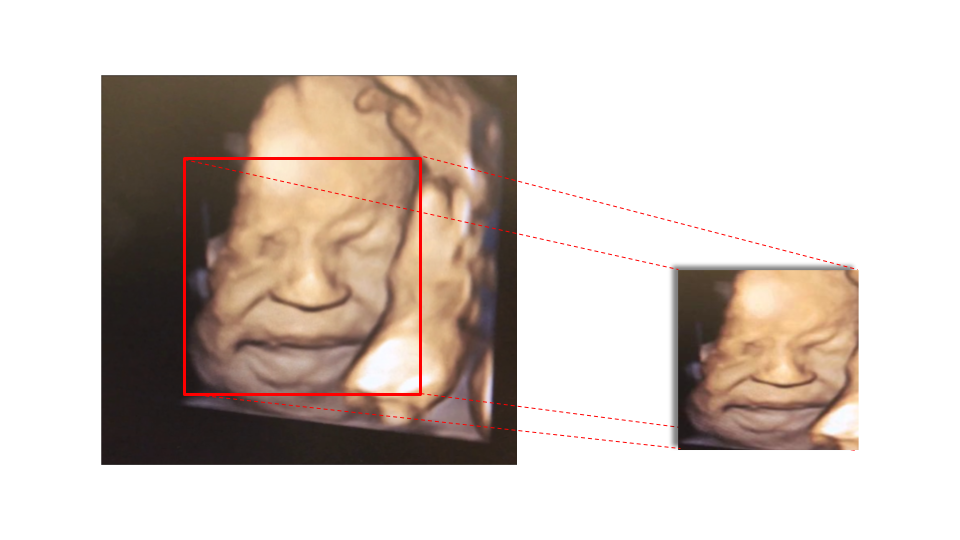
\includegraphics[width=.9\textwidth]{imgs/chap3_cropping.png}
    \caption{Image cropping with MTCNN}
    \label{fig:cropping}
\end{figure}

\subsection{Data Augmentation}

Even though we had increased the size of the dataset by turning the videos into images, it could still be considered a small dataset for deep learning models. To further augment our chances of succeeding, we have applied the use of data augmentation techniques to increase the variability of our data. The effectiveness of such a technique has been demonstrated by \cite{abs-1712-04621} and is widely used in the field.

There is a range of possibilities for using data augmentation, the ones we've chosen are:

\begin{itemize}
    \item Horizontal flip, which consists of mirroring the image horizontally. 
    \item Rotation, which consists in applying small rotations to the image.
    \item Zoom, which consists of zooming in the image.
    \item Lightning, which consists of changing the brightness and the contrast of the image.
    \item Warping, which consists of adding distortions to the image. 
\end{itemize}

All of these methods have a probability of being applied and can be used in combination with each other. Thus for each image, given the probability, a combination of these techniques would be applied. Some examples of these different combinantions of data augmentation with the same image are shown on Figure \ref{fig:data_augmentation}.

\begin{figure}[h!tp]
    \centering
    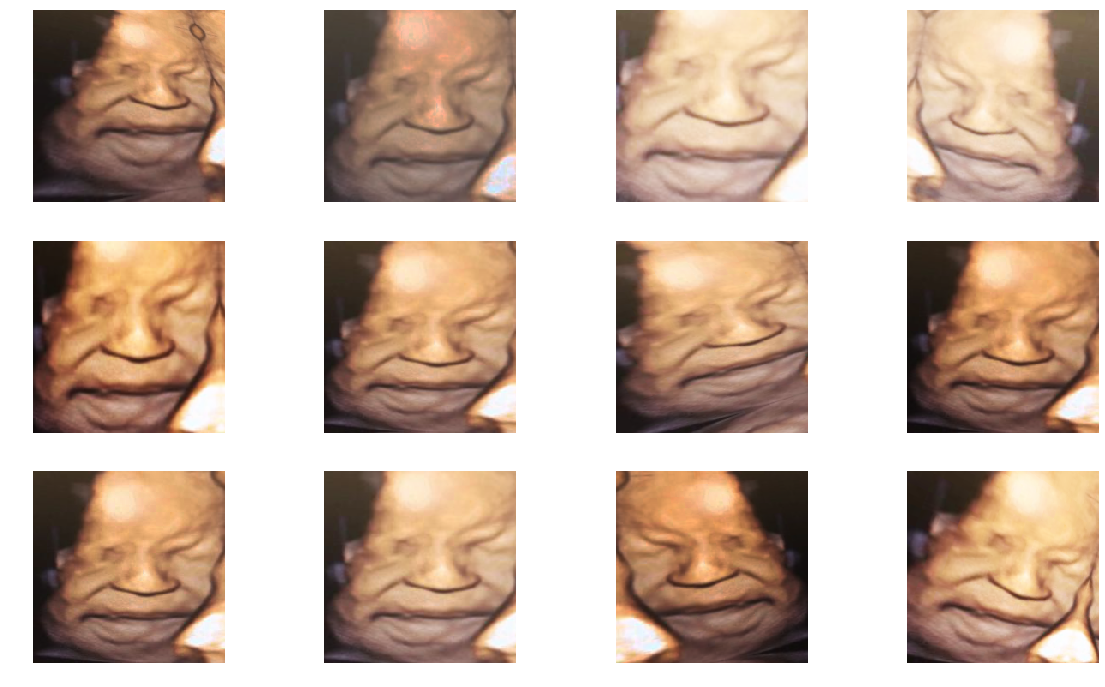
\includegraphics[width=.9\textwidth]{imgs/chap3_data_augmentation.png}
    \caption{The same image with different data augmentation applied}
    \label{fig:data_augmentation}
\end{figure}

To further experiment with this process, we have compared 3 sets of intensity in the changes. A smooth, which does more subtle changes, a medium one, which intensifies a little bit and a more aggressive one, which heavily transforms the images.  
\subsection{Network Architecture and Transfer Learning}

The network used was VGG with a pre-trained model on VGG Face, developed by \cite{ParkhiVZ15}.




\chapter{Deep Learning Models for Fetal Pain Assessment}

% In this chapter, we present some background topics recommended for a better understanding of our work and later explain the methodology that was used to conduct our experiments.

% \section{Methodology}

Based on the techniques mentioned in Chapter 3, we have proposed a learning model for classifying between images of fetuses with facial expressions indicative of pain or not. In summary, our proposed pipeline consists of sampling the videos into frames, finding the images which contain a clear fetus face, and training a CNN in with the binary classification task of finding the presence of pain. In the following sections, we describe each of these steps.

\section{Image Sampling}

It is common to have a small number of data to work within the medical field, given the inherent difficulty of collecting it. In our case, especially, only a small percentage of pregnancies require intra-uterus intervention before birth, and thus fetal anesthesia is a relatively rare procedure. 

Thus, we ended up with 15 videos available. However, it is relatively common for studies in the field to also have a small N, as mentioned by \cite{ZamzmiPGKSA16}.

Since we had such a small number of videos, it was not possible to work with them directly. So, we decided to bring the data to another dimension, reducing the space from videos to images. In order to do this, we decided to sample the videos and capture frames at a rate of 2 seconds. 

With this process, we generated a total of 708 images, but since the images were recorded from ultrasound machines, they depend on the calibration by the doctors to capture the exact section of the 3-D space where the fetus's face is clear. Because of this, it was common to find parts of the video where the face of the fetus was not visible and showed non-distinguishable parts.

As we had a significant number of images, and manual selection would be not only hard but also dependent on the observant, this became a problem.

To overcome this issue, we decided to use another neural network capable of detecting facial landmarks, like the nose, the mouth, and the eyes. The network we used was the Multi-task Cascaded Convolutional Networks (MTCNN) developed by \cite{ZhangZL016}, which identifies faces in images. It worked surprisingly well in our domain, even though the images had quite different characteristics.

With this process, we were able to filter out our dataset of images from 708 to 357 and be sure the images contained a clear face. The network returns a confidence number of which it found the face in the image, and we have used only confidences of over 95\%, which on manual inspection showed to be very reliable, with just six clear errors that were removed manually.

The position of the facial landmarks allowed us to crop the images around the face of the fetus, which is done just by adding padding to the places where they were. This process is achievable after we have the positions of the landmarks returned through the MTCNN, which also makes face alignment possible. This helps to discard images with blurred surroundings around the fetus, which contains non-distinguishable parts.  Figure \ref{fig:cropping} shows an example of a cropped image.

\begin{figure}[h!tp]
    \centering
    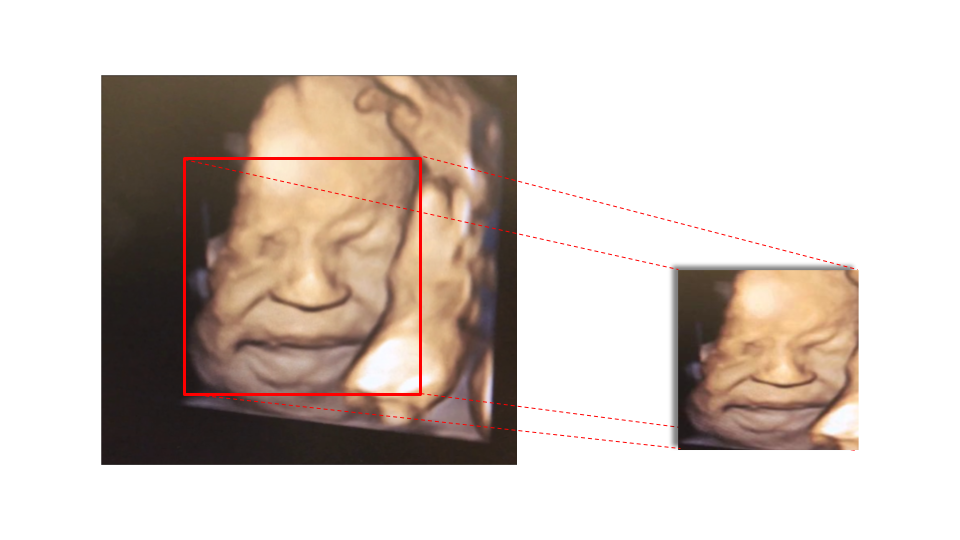
\includegraphics[width=.9\textwidth]{imgs/chap3_cropping.png}
    \caption{Image cropping with MTCNN}
    \label{fig:cropping}
\end{figure}

At this point, manual selection was needed in other to separate the images back into the three groups. With the resting images, it was easy as all the frames were from resting positions. However, with the anesthesia and horn ones, we had to split the data between before and after the stimulus. This was not a complicated process as we knew precisely when the stimuli were applied, and a clear difference in the facial expression could be noted.

\section{Data Augmentation}

Even though we had increased the size of the dataset by turning the videos into images, it is still considered a relatively small dataset for deep learning models. To further augment our chances of succeeding, we have applied the use of data augmentation techniques to increase the variability of our data. The effectiveness of this technique has been demonstrated by \cite{abs-1712-04621} and is widely used in the field.

There is a wide variety of transformations possible for using data augmentation, and the most straightforward ones usually work very well. We have chosen the following:

\begin{itemize}
    \item Horizontal flip, which consists of mirroring the image horizontally. 
    \item Rotation, which consists in applying small rotations to the images.
    \item Zoom, which consists of zooming in the image.
    \item Lightning, which consists of changing the brightness and the contrast of the image.
    \item Warping, which consists of adding distortions to the image. 
\end{itemize}

All of these methods have a probability of being applied and can be used in combination with each other. Thus for each image, given the probability, a combination of these techniques would be applied. Some examples of these different combinations within the same image are shown in Figure \ref{fig:data_augmentation}.

\begin{figure}[h!tp]
    \centering
    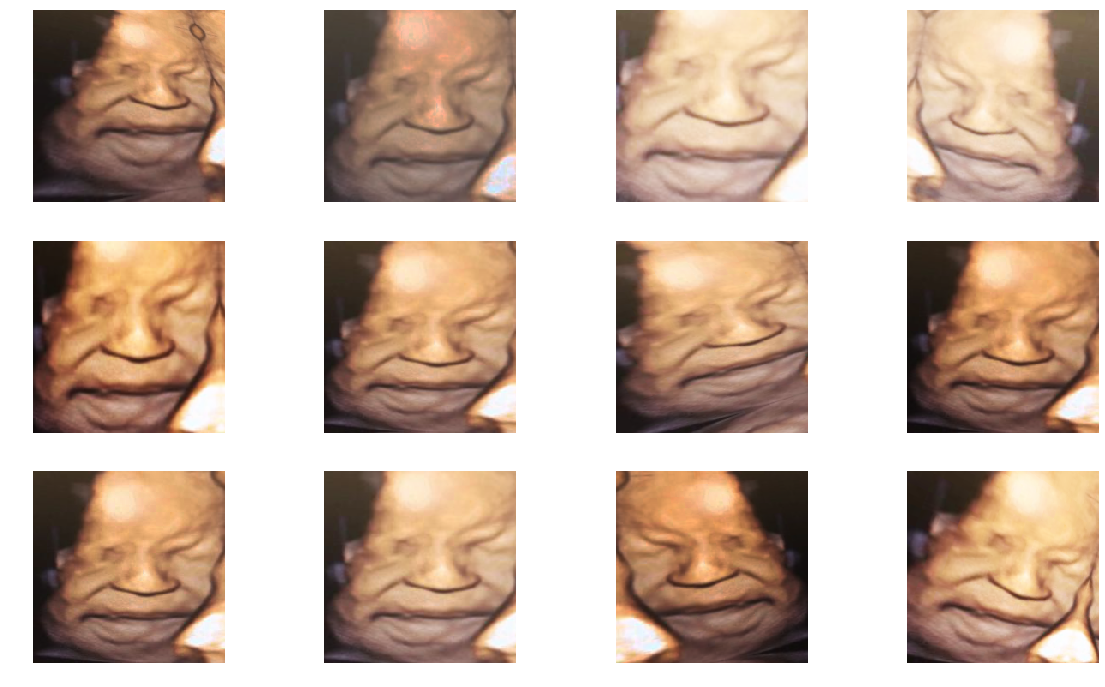
\includegraphics[width=.9\textwidth]{imgs/chap3_data_augmentation.png}
    \caption{The same image with different data transformations applied}
    \label{fig:data_augmentation}
\end{figure}

To further experiment with this process, we have compared three levels of intensity in the changes, a smooth one, which does more subtle changes, a medium one, which intensifies a little bit and a more aggressive one, which applies substantial transformations to the images.

\section{Network Architecture}

The network used was a ResNet pre-trained on the VGG Face 2 dataset, created by \cite{ParkhiVZ15}.

\section{Transfer Learning}

% The loss function we used was binary cross-entropy, as it shows good performance for classification problems with two classes. This loss function is given by the following formula:

% where λ is the set of weights, n is the number of samples in the batch, yi is the true output of the ith patient, pi is the predicted output for the ith patient, and k is the number of neurons to regularize. We optimize the network weights using Adam [Kingma and Ba, 2014], a stochastic optimization method with adaptive momentum, that is able to quickly achieve low error on the training set.



\chapter{Experimental Results}

In this chapter, we present the experimental results of our research. As no previous work has attempted to develop models for automatic pain assessment in fetuses, we have no baseline to compare to. Thus, we discuss the decisions we have made along the way, which led to our best results. In particular, our experiments aim to answer the following research questions:

\begin{itemize}
    \item \textbf{RQ1:} Is it possible to identify the presence of pain in images of fetuses from 4-D ultrasound machines? Can we create an effective learning model for automatic pain identification?
    
    \item \textbf{RQ2:} Is this model capable of discriminating images of fetuses while in acute pain exposure from those in a control group while in rest our in a non-painful sound stimulus?
    
    \item \textbf{RQ3:} Does transfer learning transfer well from a face recognition task in adults to our domain with fetuses?
\end{itemize}

\section{Setup}

Given we had relatively few data available, we chose a validation strategy that works best in this scenario. Like \cite{CelonaM17}, we used the leave-one-out method for cross-validation, but instead of leaving one image out, we leave one subject. Hence, we produce 13 different combinations containing training and test subsets. On each of these combinations, we train our networks in the training subset with images of twelve fetuses and evaluate on the test subset with images of one. All the evaluations are then averaged to assess the overall performance of the models.

In order to find the best network architecture for this particular problem, we have tested a few variations in the setup as described in Chapter 5. These variations are regarding three variables:

\begin{itemize}
    \item Data augmentation, which could be with weak or strong transformations.

    \item Network training, which could be with frozen or unfrozen layers.

    \item Pre-training, which could be on the ImageNet or the VGGFace2 datasets.
\end{itemize}

By combining all the possibilities of these three variables, we have a total of eight experiments. Like \cite{abs-1807-01631}, we have chosen two types of pre-training for the CNNs, so we can compare the differences between using CNNs trained on a relatively similar dataset like VGGFace2, as opposed to CNNs trained on a general-purpose dataset like ImageNet.

Besides these variations, all the networks used Adam as a gradient descent optimization algorithm \citep{KingmaB14}, which uses adaptive momentum to reduce the error in the training set quickly. We have used a batch size of 8 for both training and validation, which yielded the best results after we have experimented with different sizes (4, 8, 16, 24). We have also applied some methods to prevent over-fitting like L2 for weight regularization \citep{Ng2004} and dropout \citep{SrivastavaHKSS14}. Lastly, the loss function we used was binary cross-entropy, as it shows good performance for classification problems with two classes.

The metric we used to evaluate our model during the validation process was accuracy. To calculate it for a given test set, we divide the number of images we have predicted the correct class by the total number of images available in that set.

Additionally, we have also calculated another metric for the videos of acute pain (AP). As we have 45 seconds of video before the acute pain stimulus, and 45 seconds after it, we have images from both classes in these videos: pain and non-pain.  This division allows the use of a metric that considers not only the cases we are making the correct prediction but also how much of each class we are making the wrong predictions. Thus, like \cite{abs-1807-01631}, we have used the Area Under the Receiver Operating Characteristic Curve (AUC) to evaluate the performance of our models in the set of acute pain videos.

\section{Results}

In this section, we compare the performance of each training approach and discuss their results. Table \ref{tab:accuracy_all} displays the results in terms of accuracy considering each training method, which gives us some insights about the behavior of the different models. For instance, we can see our best result came from a pre-training on VGGFace2, which confirms our hypothesis that it was better to use pre-training on a set of images similar to ours and that the features learned from these images transfer well to fetuses.

However, when looking at all the results, we can see that the overall standard deviation was reasonably high, which shows how challenging the task is when we have little data. In fact, by looking only at the dimensions of training type and transformations, a clear winner approach is not evident, as the results are very similar and one variation not always perform better than the other.

\begin{table}[h!tp]
\centering
\caption{Accuracy comparison considering all videos.}
\label{tab:accuracy_all}
\begin{tabular}{lllll}
\toprule
         &        &          & \multicolumn{2}{l}{Accuracy} \\
         &        &          &     Mean &    Std \\
Training & Transforms & Network &          &        \\
\midrule
freeze   & weak   & ResNet (ImageNet) &    0.778 &  0.267 \\
freeze   & weak   & ResNet (VGGFace2) &    0.721 &  0.275 \\
freeze   & strong & ResNet (ImageNet) &    0.671 &  0.308 \\
freeze   & strong & ResNet (VGGFace2) &    \textbf{0.787} & \textbf{ 0.231} \\
unfreeze & weak   & ResNet (ImageNet) &    0.702 &  0.273 \\
unfreeze & weak   & ResNet (VGGFace2) &    0.731 &  0.237 \\
unfreeze & strong & ResNet (ImageNet) &    0.749 &  0.243 \\
unfreeze & strong & ResNet (VGGFace2) &    0.727 &  0.243 \\
\bottomrule
\end{tabular}
\end{table}

When we look at the accuracy reported in each test set for the best model in Table \ref{tab:accuracy_leave_one_out}, we can see the model performs well in the acute pain (AP) and rest (RE) groups, but has a hard time predicting images from the acoustic stimulus (AS) group.

\begin{table}[h!tp]
\setlength{\tabcolsep}{3.41pt}
\centering
\caption{Accuracy per test set in the leave-one-out for the best model.}
\label{tab:accuracy_leave_one_out}
\begin{tabular}{lllllllllllll}
\hline
\multicolumn{13}{l}{Accuracy}        \\ \hline
\multicolumn{1}{l|}{$1_{AP}$}  & \multicolumn{1}{l|}{$2_{AP}$}  & \multicolumn{1}{l|}{$3_{AP}$}  & \multicolumn{1}{l|}{$4_{AP}$}  & \multicolumn{1}{l|}{$5_{AP}$}  & \multicolumn{1}{l|}{$6_{AP}$}  & \multicolumn{1}{l|}{$7_{RE}$}  & \multicolumn{1}{l|}{$8_{RE}$}  & \multicolumn{1}{l|}{$9_{RE}$}  & \multicolumn{1}{l|}{$10_{RE}$} & \multicolumn{1}{l|}{$11_{AS}$} & \multicolumn{1}{l|}{$12_{AS}$} & $13_{AS}$ \\ \hline
\multicolumn{1}{l|}{0.917} & \multicolumn{1}{l|}{0.824} & \multicolumn{1}{l|}{0.583} & \multicolumn{1}{l|}{0.875} & \multicolumn{1}{l|}{0.850} & \multicolumn{1}{l|}{0.769} & \multicolumn{1}{l|}{1.000} & \multicolumn{1}{l|}{1.000} & \multicolumn{1}{l|}{1.000} & \multicolumn{1}{l|}{0.667} & \multicolumn{1}{l|}{0.250} & \multicolumn{1}{l|}{0.500} & 1.000 \\ \hline
\end{tabular}
\end{table}

If we look at the accuracy mean of the test sets in Table \ref{tab:mean_accuracy_group}, which are grouped by the three evaluated scenarios, we can see how our score was much lower in the acoustic stimulus (AS) group than the other two. 

\begin{table}[h!tp]
\centering
\caption{Mean accuracy per image group.}
\label{tab:mean_accuracy_group}
\begin{tabular}{lc}
\hline
                       & Accuracy \\ \hline
Acute Pain (AP)        & 0.803    \\
Rest (RE)              & 0.917    \\
Acoustic Stimulus (AS) & 0.583    \\ \hline
\end{tabular}
\end{table}

This result can be explained partly because it was harder to distinguish these images from pain, as the expressions of discomfort, anger, hunger, for example, can also generate similar reactions. However, besides that, we believe the fact this group had fewer videos, and that the original videos were noisier than the other groups, could have also contributed to the lower accuracy.

Nonetheless, we can also take a closer look at the results from the acute pain (AP) group, from which we can measure the AUC. As we can see on Table \ref{tab:accuracy_auc_ap}, we have performed much better on this group, especially considering we had images of the same fetuses on both states, pain and non-pain. This result is very promising, as it indicates our model is able to discriminate pain from rest on images of fetuses.

\begin{table}[h!tp]
\centering
\caption{Accuracy and AUC considering only Acute Pain videos.}
\label{tab:accuracy_auc_ap} 
\begin{tabular}{lllllll}
\toprule
         &        &          & \multicolumn{2}{l}{Accuracy} & \multicolumn{2}{l}{AUC} \\
         &        &          &      Mean &       Std &      Mean &       Std \\
Training & Transforms & Network &           &           &           &           \\
\midrule
freeze   & weak   & ResNet (ImageNet) &  0.710 &  0.233 &  0.849 &  0.173 \\
freeze   & weak   & ResNet (VGGFace2) &  0.768 &  0.155 &  0.885 &  0.150 \\
freeze   & strong & ResNet (ImageNet) &  0.698 &  0.205 &  0.850 &  0.130 \\
freeze   & strong & ResNet (VGGFace2) &  \textbf{0.802} & \textbf{ 0.118} &  \textbf{0.923} &  \textbf{0.063} \\
unfreeze & weak   & ResNet (ImageNet) &  0.684 &  0.198 &  0.813 &  0.163 \\
unfreeze & weak   & ResNet (VGGFace2) &  0.763 &  0.132 &  0.898 &  0.112 \\
unfreeze & strong & ResNet (ImageNet) &  0.692 &  0.185 &  0.909 &  0.110 \\
unfreeze & strong & ResNet (VGGFace2) &  0.742 &  0.139 &  0.833 &  0.156 \\
\bottomrule
\end{tabular}
\end{table}

We can see that the best model is still the same as the one from Table \ref{tab:accuracy_all}. However, now we have some more insights in terms of the other two dimensions. For example, we can see that the strong transformations have a slight advantage when compared to the weak in terms of AUC. Likewise, training the network with frozen layers performs better than unfrozen in terms of accuracy, which could also be caused by the noise in the data, so the error propagates back into the first layers, causing the network to worsen its performance. Although more data would be necessary to make conclusions.

Also, we can see the standard deviation is much lower, which can be explained not only by the fact we have fewer validations sets to consider but also because our model is performing better at predicting acute pain videos.

\begin{table}[h!tp]
\setlength{\tabcolsep}{3.41pt}
\centering
\caption{AUC per test set in the leave-one-out for the best model, considering only Acute Pain videos.}
\label{tab:auc_leave_one_out}
\begin{tabular}{llllll}
\hline
\multicolumn{6}{l}{AUC} \\ \hline
\multicolumn{1}{l|}{$1_{AP}$}    & \multicolumn{1}{l|}{$2_{AP}$}    & \multicolumn{1}{l|}{$3_{AP}$}    & \multicolumn{1}{l|}{$4_{AP}$}    & \multicolumn{1}{l|}{$5_{AP}$}    & $6_{AP}$   \\ \hline
\multicolumn{1}{l|}{0.991} & \multicolumn{1}{l|}{0.983} & \multicolumn{1}{l|}{0.829} & \multicolumn{1}{l|}{0.938} & \multicolumn{1}{l|}{0.870} & 0.929 \\ \hline
\end{tabular}
\end{table}

When we look at the result from each test set of acute pain (AP) from the best model in Table \ref{tab:auc_leave_one_out}, we see that videos $3_{AP}$ and $5_{AP}$ have a lower AUC, which shows how much variations in the images can affect the final result when we work with little.

\section{Visual Explanations}

The success of convolutional neural networks came with the ever-increasing complexity of the architectures, which led to difficulties in understanding why the models make certain decisions. Some methods exist to try to overcome this issue, such as Grad-CAM \citep{SelvarajuCDVPB17}, which tries to provide visual explanations of why the model made a given decision. This method uses the gradients of the target flowing back into the final convolutional layer to produce a heat map that highlights the important regions in the image that were used for prediction.

We have attempted to use this technique to identify the parts of the image our models found that were the most relevant for classifying an image as pain. In an ideal scenario, the heat map should be stronger in the parts of the image that are indicators of pain, like the ones used by the pain scales. However, even though this did happen for some examples, as we can see in Figure \ref{fig:gradcam}, for most cases, the heat map was inconclusive. We believe this could also be an effect of the limited amount of data, thus we propose this topic gets further investigated in a future work.

\begin{figure}[h!tp]
    \centering
    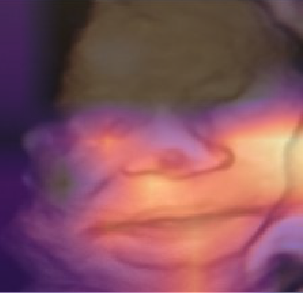
\includegraphics[width=0.4\textwidth]{imgs/chap6_gradcam.png}
    \caption{Grad-CAM heat map for visual explanations.}
    \label{fig:gradcam}
\end{figure}

\section{Answering Our Research Questions}

In this section, we aim to answer the proposed research questions from the beginning of this chapter based on the results we presented.

Regarding \textbf{RQ1}, we believe our results showed in tables \ref{tab:accuracy_all} and \ref{tab:accuracy_auc_ap} are a good argument to show it is viable to develop a learning model capable of effectively identifying pain. We believe an accuracy of 0.787 is good evidence we are in the right direction, even considering that a new experiment with more data could be necessary to validate these conclusions further. As data is complicated to collect, we think our experimental process was able to extract significant results out of it.

As for \textbf{RQ2}, we did see our model had problems in discriminating images of acute pain from those of an acoustic stimulus, although it did so very well from images of rest. It appears the images from acoustic stimulus indeed made the task more difficult, but we believe this effect would be mitigated if we had a larger dataset available for training. Nevertheless, even if we have a false positive predicted from an acoustic stimulus image, from a precautionary perspective, it would still benefit the fetus, as this could be an indication of discomfort and could also be treated.

Finally, for \textbf{RQ3}, it does appear transfer learning with pre-training in the VGGFace2 dataset performs better than when trained on ImageNet, as it achieved our best result. We believe this comes from the fact the pre-training on face images was able to learn features in their middle to last layers related to the human face, such as the mouth, the eyes, the chin, the nose. Even though the fetus images are relatively different, these features are still present, which could explain why this model detected them and performed better. 


\chapter{Conclusions and Future Work}

\section{Conclusions}

The results of our study presented in this dissertation are promising as we believe they move us towards the ultimate goal of automatically detecting pain in fetuses. Our learning model was indeed able to discriminate images of fetuses while in acute pain exposure from those in control groups of rest and acoustic stimulus. If confirmed on a larger dataset, we believe this work has the potential to influence and improve the current practice of assessing fetal pain.

We also think our work can serve as good evidence to help answer the question of when fetuses start to feel pain, as the exact gestational week in which they start showing pain responses is still not a consensus. By providing an unbiased and automatic approach for detecting pain, we could continuously monitor a fetus across many weeks, and an absence of pain may even be a good indicator of fetal wellbeing. However, a dataset with more variable gestational age would be necessary to train such a model.

On the other hand, if we do detect pain, the question arises as to what is the cause of it, as some condition may be present since our model accused the presence of pain. Is this condition some malformation? Is it a disease? Or is it related to chronic pain? It does open a range of possibilities but also brings awareness to future problems, which in some cases could be corrected with in-uterus repairs, with many benefits for the fetus.

As for the control group of acoustic stimuli, our model found it more difficult to discriminate it from pain, which was an expected outcome.  Because the group shares some common indicators with those of pain, it makes it indeed harder to predict, as shown in the original study that collected the data \citep{bernardes2018feasibility}. Nonetheless, we still believe that from a precautionary approach, it may be a good practice to investigate these cases, as they can be signs of discomfort or stress, and may also be caused by some conditions.

If our model eventually gets integrated into an ultrasound machine, it would make pain detection much simpler and easier to use, allowing continuous monitoring. This would be beneficial in many situations, especially during fetal surgery procedures, as it could aid anesthesiologists to see how effective their anesthesia was and aid the doctors while they perform the delicate procedures. Likewise, during routine prenatal ultrasound exams, this system could be the first to indicate pain or discomfort, which would then be further investigated.

It is also important to highlight that even though nurses and caregivers must assess the videos used as inputs by our model, we think a model trained on a range of different videos from different sources, would tend to be much more unbiased than an assessment of a single caregiver. This result is also a great benefit, as we can produce a system ideally free from bias factors such as identity, background, culture, and gender, which may lead to inconsistent assessment and treatment of pain.

\section{Future Work}

Our studies have shown that it is viable to construct a model capable of identifying the presence of pain on images of fetuses from 4-D ultrasound machines. A larger dataset is already being collected by the same fetal pain study group, which has the potential to confirm our results and produce models that are even more robust and accurate. We are also currently not able to explain why the model made such predictions or what is the main factors it considered for detecting pain. Thus, we identify as future work the following possibilities:

\begin{itemize}
    \item Evaluate our models on larger datasets. Even though the data is quite complicated to collect and studies with fetuses and infants usually have a small number of subjects, we think it would be very beneficial to experiment with our methodology in a more extensive number of fetuses. This addition could bring more variability into the model inputs in terms of fetal positions, gestational age, gender, image quality, and many other factors, which will end up producing a better model.
    
    \item Expand our system to include chronic pain. Monitoring the same fetuses at different gestational ages has the potential to identify the presence of chronic factors. A model that evaluates not only acute pain but also chronic pain could, therefore, help in this scenario, as it may lead to further investigation of what is causing the chronic pain and maybe be the first indicator that an intervention may be necessary.

    \item Include other types of features. As it is the case with pain scales, the combination of indicators is what tends to work best. Thus one could construct a model that takes as inputs not only images of the face and facial expressions but also other indicators such as sounds, body movements, physiological indicators, and biological markers. These new factors could help produce more robust models, and maybe identify conditions not visible through facial expressions only.
    
    \item Produce explainable models. Given a single fetus where the presence of pain has been identified, one should be able to visualize what are the most relevant features that the model analyzed to output its prediction. By making the decision of the models more transparent, one could point to the exact locations where the pain was present, which will lead to a better understating by fetal pain specialists. In an ideal scenario, these visual explanations should match the individual indicators present on the pain scale.

\end{itemize}

In summary, our main interests as future works are to help medical experts to understand the output of the models better and be more effective on pain assessment and management, which will eventually lead into improving overall fetuses life quality and well-being.

% Aqui vem a parte da bibliografia: use o comando \ppgccbibliography indicando
% apenas o nome do arquivo .bib (sem a extensão).
\ppgccbibliography{bibfile}

\end{document}
